\documentclass[UTF8,zihao=-4]{ctexart}

\usepackage[a4paper,margin=1.8cm]{geometry}
\usepackage{booktabs}
\usepackage{graphicx}
\usepackage{caption}
\usepackage{longtable}
\usepackage{pdflscape}
\usepackage{ragged2e}
\usepackage{xcolor}
\usepackage[colorlinks=true,citecolor=blue!55!black,urlcolor=blue!55!black]{hyperref}
\usepackage[backend=biber,style=apa,sorting=nyt]{biblatex}

\addbibresource{references.bib}
\setlength{\parindent}{2em}
\setlength{\parskip}{0.25em}

\title{Supplementary information for ChinaTherm30}
\author{}
\date{}

\begin{document}
\maketitle

\renewcommand{\thefigure}{S\arabic{figure}}
\renewcommand{\thetable}{S\arabic{table}}

\section*{Supplementary Figures}

\begin{figure}[p]
\centering
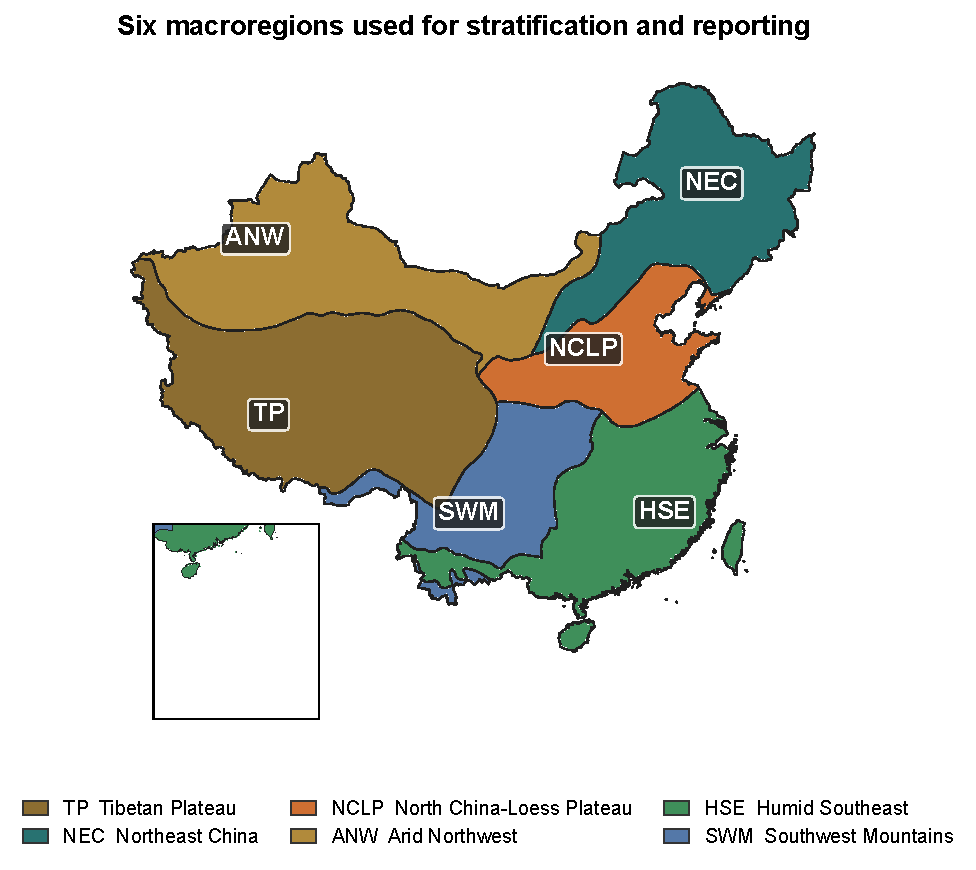
\includegraphics[width=0.96\linewidth]{../figures/FigureS1.pdf}
\caption{Six macroregions used for stratified sampling and regional reporting. The boundaries aggregate 46 ecological regions from the China eco-geographical regionalization: TP, Tibetan Plateau; NEC, Northeast China; NCLP, North China--Loess Plateau; ANW, Arid Northwest; HSE, Humid Southeast; and SWM, Southwest Mountains. These abbreviations are used consistently in the main text and figures.}
\label{fig:s1-macroregions}
\end{figure}

\clearpage
\begin{figure}[p]
\centering
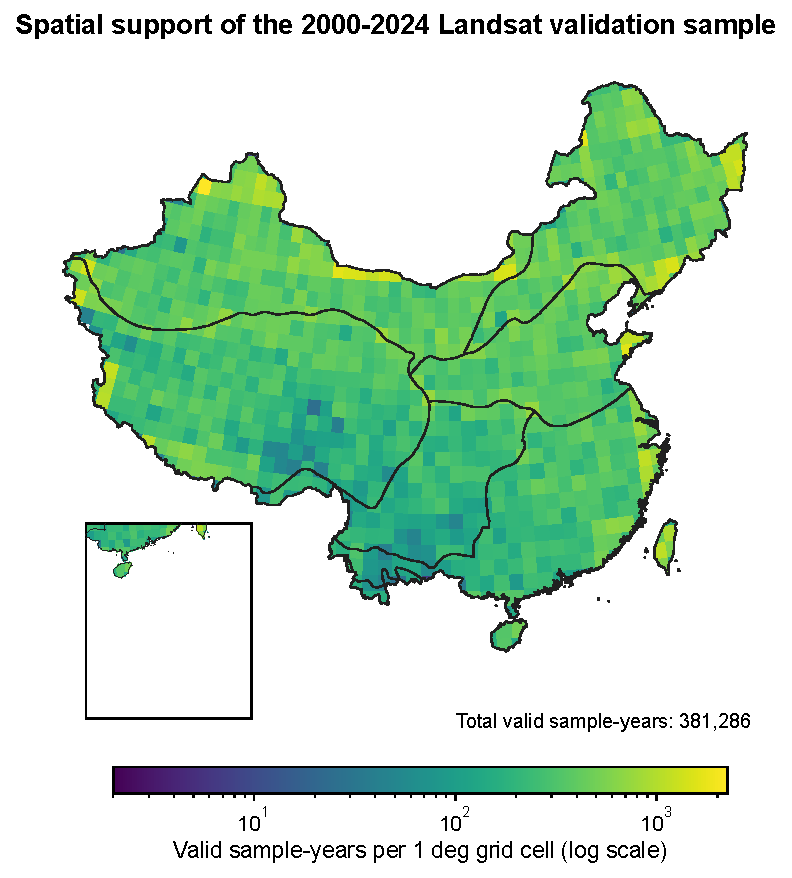
\includegraphics[width=0.96\linewidth]{../figures/FigureS2.pdf}
\caption{Spatial support of the nationwide Landsat Collection 2 surface-temperature validation. Valid samples from 2000--2024 are aggregated to 1° grid cells to avoid overplotting. A sample-year requires strict cloud, shadow, snow and radiometric-saturation screening, at least three valid Landsat observations, available 3$\times$3 ChinaTherm30 and RF-LST baseline means, and a water fraction no greater than 10\%. Macroregion boundaries follow Figure~S1.}
\label{fig:s2-landsat-density}
\end{figure}

\clearpage
\begin{figure}[p]
\centering
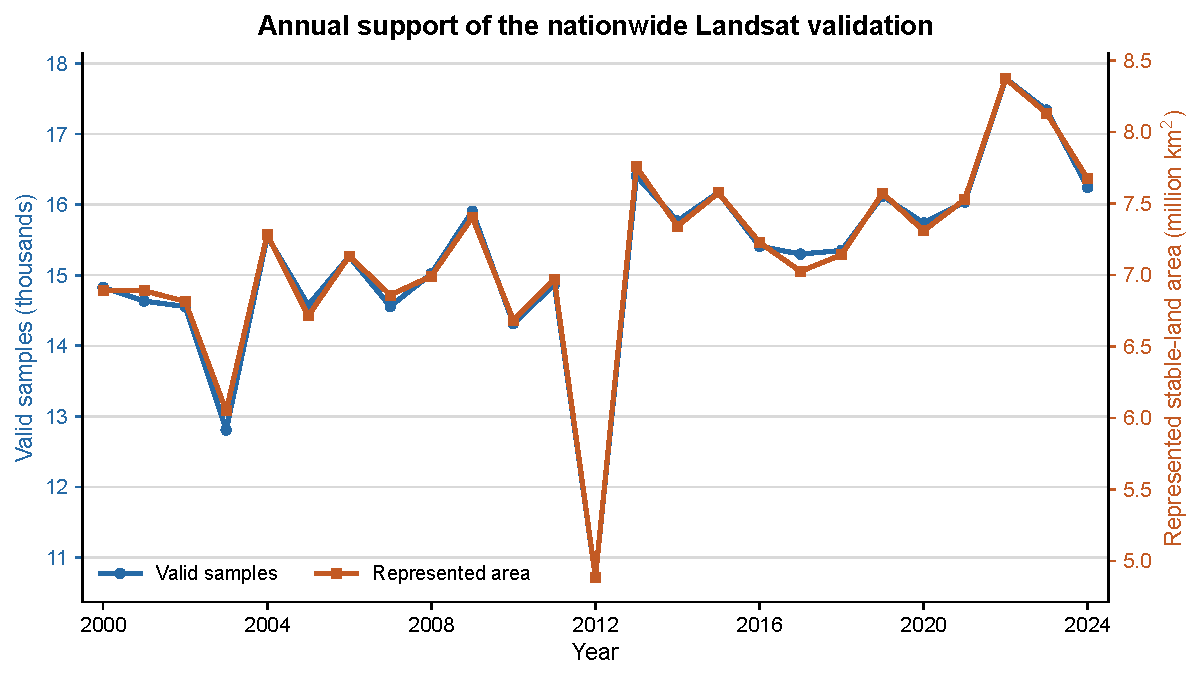
\includegraphics[width=0.94\linewidth]{../figures/FigureS3.pdf}
\caption{Annual support of the nationwide Landsat validation. Valid sample counts and represented stable-land area use the same eligibility and analysis weights as the area-weighted validation metrics in the main text.}
\label{fig:s3-landsat-annual}
\end{figure}

\clearpage
\begin{figure}[p]
\centering
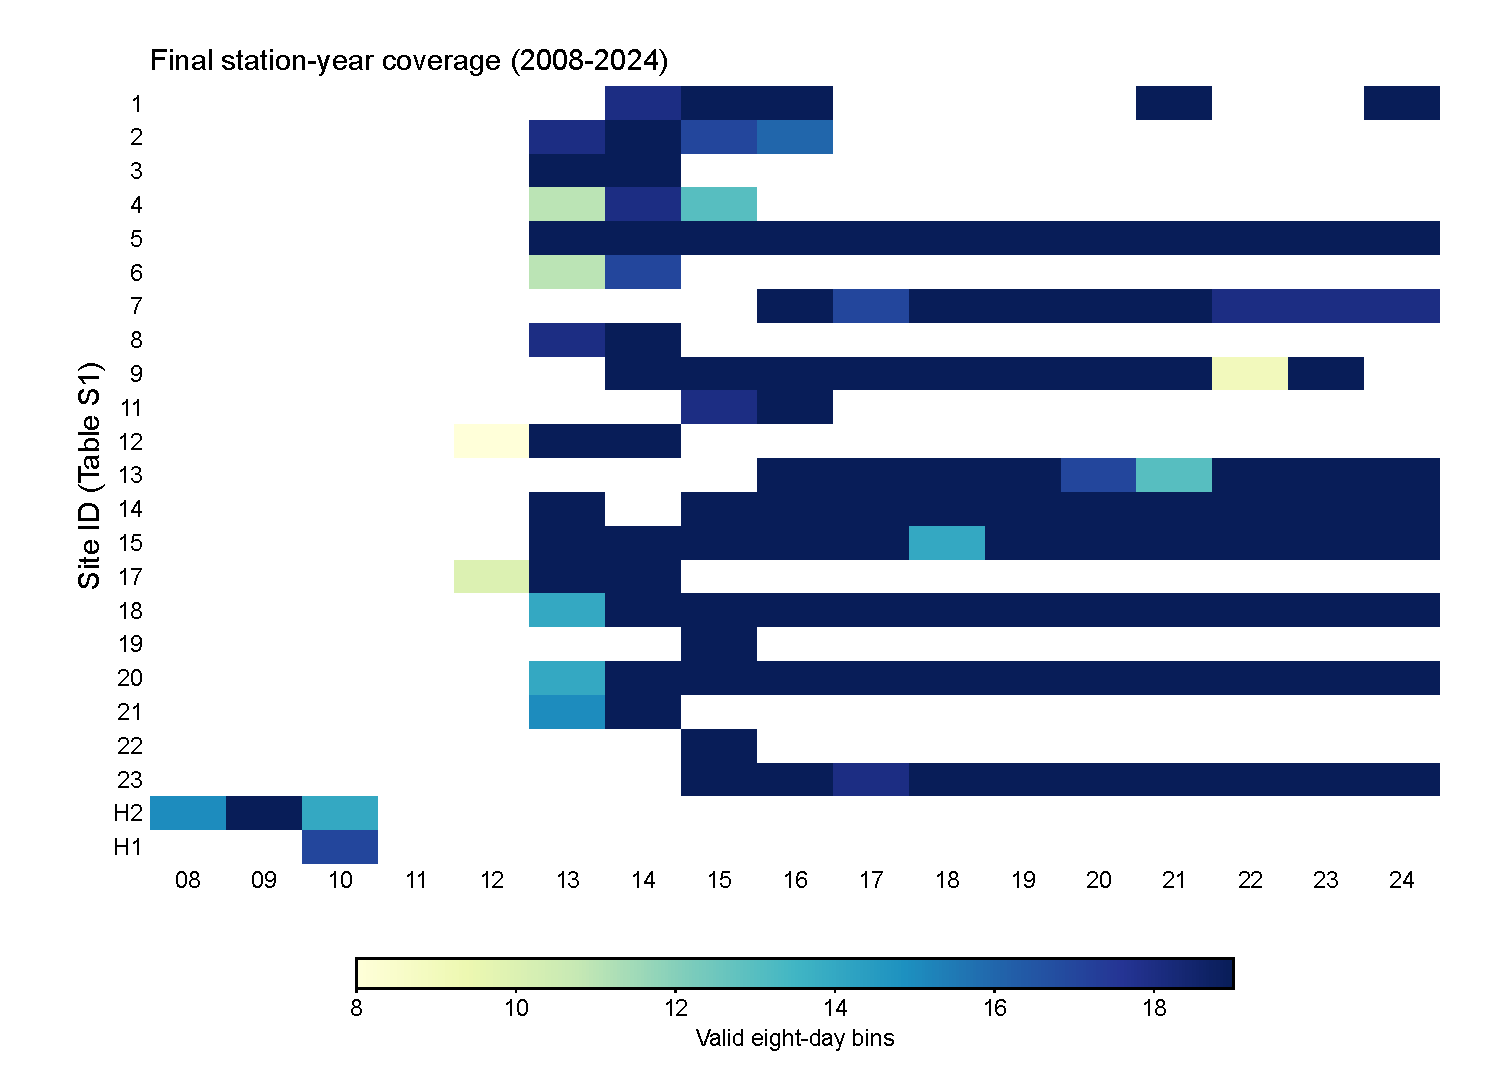
\includegraphics[width=0.94\linewidth]{../figures/FigureS4.pdf}
\caption{Temporal coverage of the final ground-validation set. Colours indicate the number of valid MOD11A2-aligned eight-day bins contributing to each station-year annual IRT composite. The final set contains 131 station-years across all 23 sites and 16 calendar years. Site IDs follow Table~S1.}
\label{fig:s4-ground-coverage}
\end{figure}

\clearpage
\begin{figure}[p]
\centering
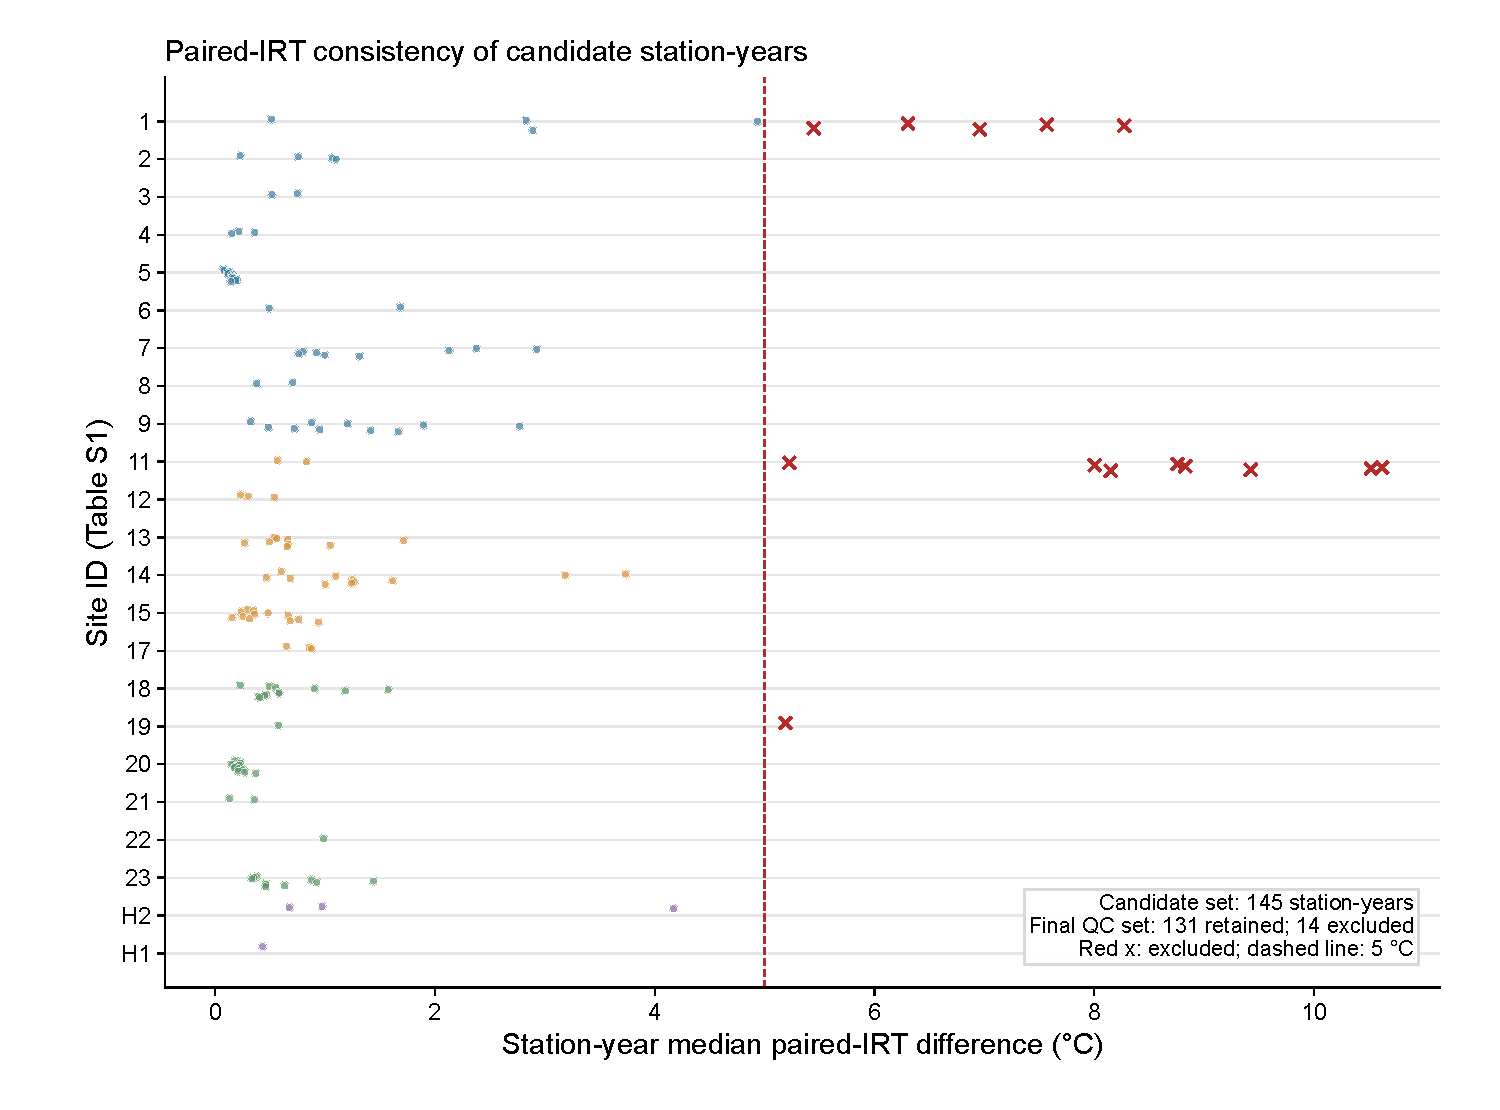
\includegraphics[width=0.94\linewidth]{../figures/FigureS5.pdf}
\caption{Paired-IRT consistency within the 145 candidate station-years. A paired-sensor diagnostic was available for 143 records. Fourteen station-years with a median daily paired-IRT absolute difference greater than 5~$^{\circ}$C were excluded from the final ground-reference set; the remaining 131 station-years retained all 23 sites. The criterion uses only ground-sensor measurements.}
\label{fig:s5-ground-qc}
\end{figure}

\clearpage
\begin{figure}[p]
\centering
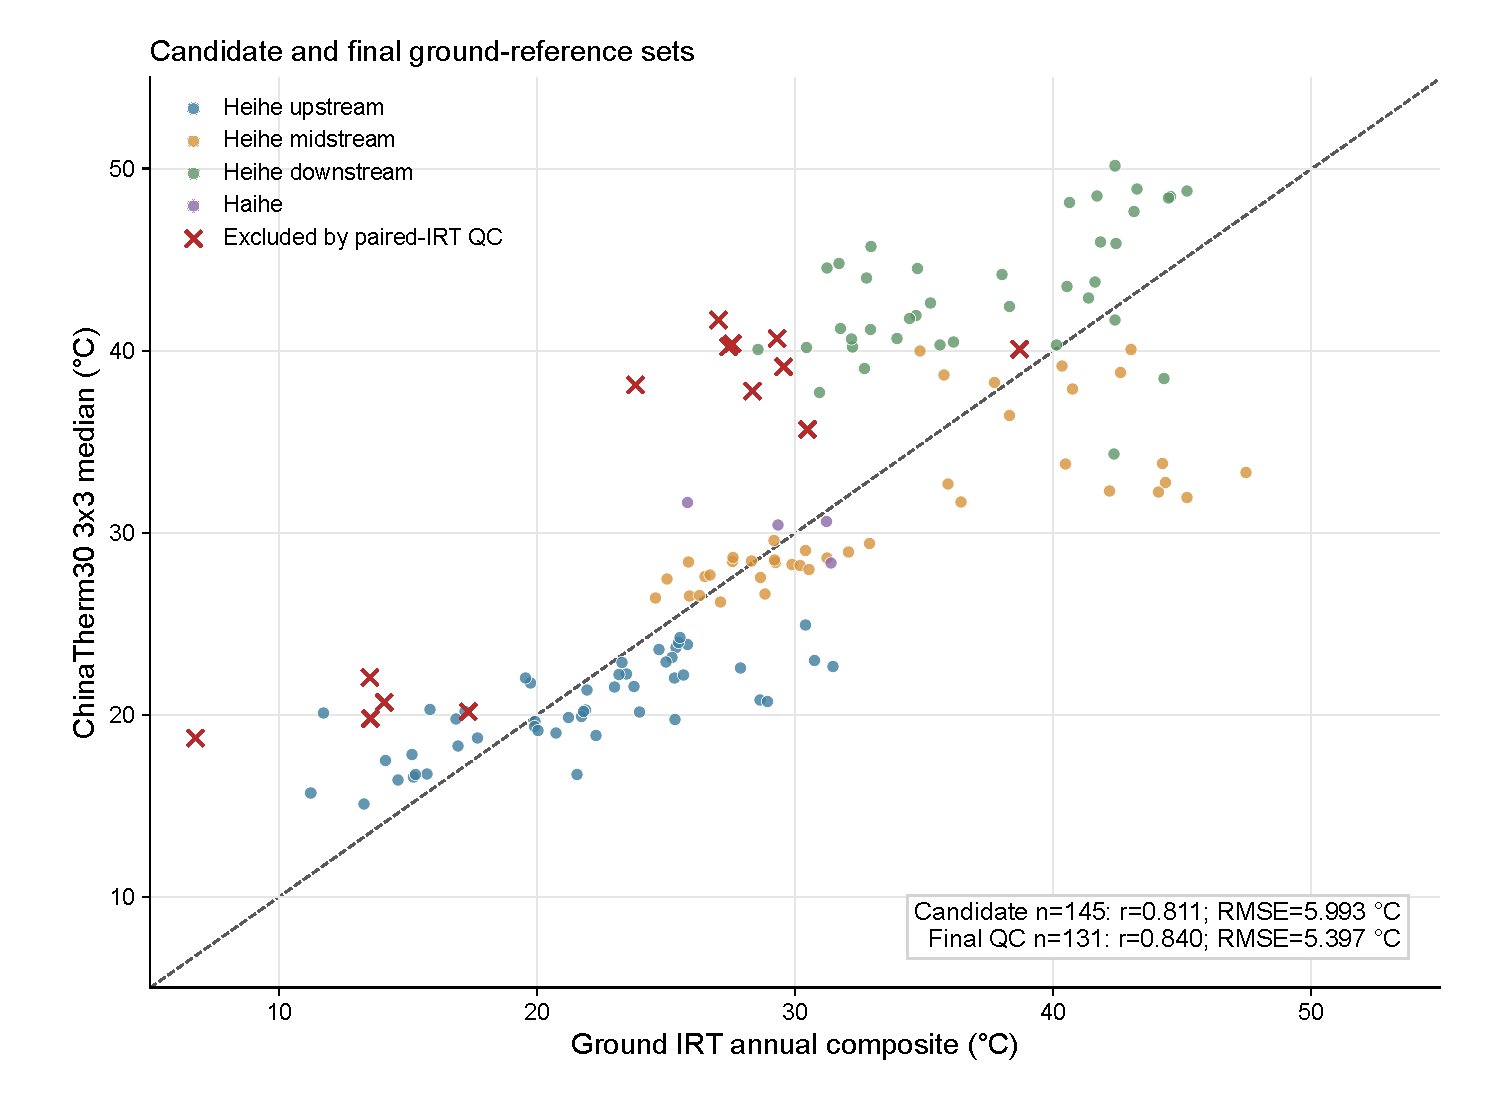
\includegraphics[width=0.92\linewidth]{../figures/FigureS6.pdf}
\caption{ChinaTherm30 3$\times$3 neighbourhood medians compared with annual ground-IRT composites before and after ground-reference quality control. Coloured circles are the 131 final station-years, and red crosses are the 14 records excluded by the paired-IRT criterion. Summary statistics report the complete 145-record candidate set and the 131-record final set.}
\label{fig:s6-ground-set-comparison}
\end{figure}

\clearpage
\begin{figure}[p]
\centering
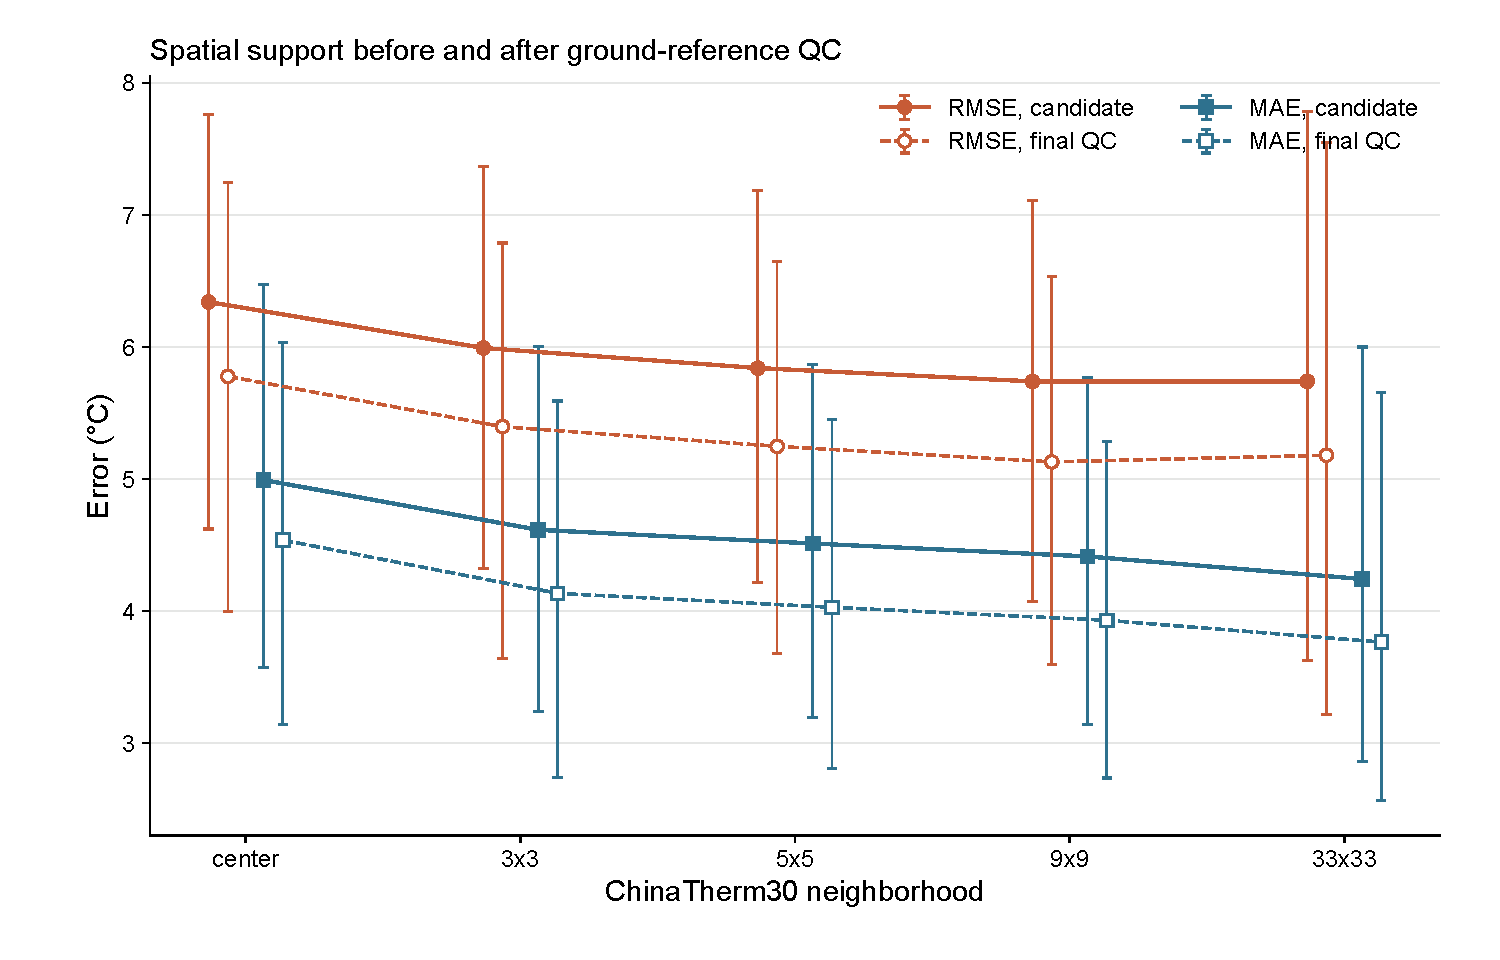
\includegraphics[width=0.94\linewidth]{../figures/FigureS7.pdf}
\caption{Spatial-support sensitivity before and after ground-reference quality control. Points show RMSE and MAE for the ChinaTherm30 centre pixel and median neighbourhoods from 3$\times$3 to 33$\times$33 pixels; error bars are 95\% site-cluster bootstrap intervals. The four series are slightly offset horizontally within each neighbourhood for legibility. The main text reports the final quality-controlled set.}
\label{fig:s7-ground-support}
\end{figure}

\clearpage
\begin{landscape}
\section*{Supplementary Tables}
\scriptsize
\setlength{\tabcolsep}{2.4pt}
\renewcommand{\arraystretch}{1.12}
\begin{longtable}{@{}c p{2.8cm} p{1.1cm} p{1.35cm} p{2.35cm} r r r p{2.25cm} r p{1.25cm} r p{1.95cm}@{}}
\caption{Station metadata, source parsing, and final validation coverage. Heihe Site IDs 1--23 follow \textcite{liu2018heiheNetwork}; H1 and H2 denote the Guantao and Daxing sites in the Haihe basin. Candidate records use $K\geq0.65$, 10:30 local mean solar time $\pm30$ min, and at least eight valid MOD11A2-aligned eight-day bins; final coverage additionally applies the paired-IRT ground-reference criterion.}\label{tab:s1-stations}\\
\toprule
\shortstack{Site\\ID} & Station & Network & Reach & Landscape & Lon. & Lat. & Elev. & \shortstack{Duration\\reported} & \shortstack{Parsed\\XLSX} & \shortstack{Final\\years} & \shortstack{Site-\\years} & Status \\
\midrule
\endfirsthead
\multicolumn{13}{l}{\textit{Table S1 continued}}\\
\toprule
\shortstack{Site\\ID} & Station & Network & Reach & Landscape & Lon. & Lat. & Elev. & \shortstack{Duration\\reported} & \shortstack{Parsed\\XLSX} & \shortstack{Final\\years} & \shortstack{Site-\\years} & Status \\
\midrule
\endhead
\midrule
\multicolumn{13}{r}{\textit{Continued on next page}}\\
\endfoot
\bottomrule
\endlastfoot
1 & Jingyangling & Heihe & Up. & alpine meadow & 101.120 & 37.840 & 3750 & Aug. 2013-present & 13 & 2014-2024 & 5 & Final QC \\
2 & E'bao & Heihe & Up. & alpine meadow & 100.920 & 37.950 & 3294 & June 2013-Oct. 2016 & 4 & 2013-2016 & 4 & Final QC \\
3 & Huangcaogou & Heihe & Up. & alpine meadow & 100.730 & 38.000 & 3137 & June 2013-Apr. 2015 & 4 & 2013-2014 & 2 & Final QC \\
4 & Arou Sunny & Heihe & Up. & alpine meadow & 100.520 & 38.090 & 3529 & Aug. 2013-Aug. 2015 & 3 & 2013-2015 & 3 & Final QC \\
5 & Arou & Heihe & Up. & subalpine meadow & 100.460 & 38.050 & 3033 & June 2008-present & 12 & 2013-2024 & 12 & Final QC \\
6 & Arou Shady & Heihe & Up. & alpine meadow & 100.410 & 37.980 & 3536 & Aug. 2013-Aug. 2015 & 3 & 2013-2014 & 2 & Final QC \\
7 & Yakou & Heihe & Up. & alpine meadow & 100.240 & 38.010 & 4148 & Jan. 2014-present & 10 & 2016-2024 & 9 & Final QC \\
8 & Huangzangsi & Heihe & Up. & wheat & 100.190 & 38.230 & 2612 & June 2013-Apr. 2015 & 4 & 2013-2014 & 2 & Final QC \\
9 & Dashalong & Heihe & Up. & alpine marsh & 98.940 & 38.840 & 3739 & Aug. 2013-present & 12 & 2014-2023 & 10 & Final QC \\
10 & Guantan & Heihe & Up. & Qinghai spruce & 100.250 & 38.530 & 2835 & 2008-2011 & 0 & -- & 0 & No IRT workbook \\
11 & Huazhaizi & Heihe & Mid. & Kalidium desert & 100.320 & 38.770 & 1731 & June 2012-present & 12 & 2015-2016 & 2 & Final QC \\
12 & Shenshawo & Heihe & Mid. & sandy desert & 100.490 & 38.790 & 1594 & June 2012-Apr. 2015 & 4 & 2012-2014 & 3 & Final QC \\
13 & Heihe RS & Heihe & Mid. & grassland & 100.480 & 38.830 & 1560 & Aug. 2014-present & 9 & 2016-2024 & 9 & Final QC \\
14 & Zhangye wetland & Heihe & Mid. & reed & 100.450 & 38.980 & 1460 & June 2012-present & 11 & 2013-2024 & 11 & Final QC \\
15 & Daman & Heihe & Mid. & maize & 100.370 & 38.860 & 1556 & May 2012-present & 12 & 2013-2024 & 12 & Final QC \\
16 & Yingke & Heihe & Mid. & maize & 100.410 & 38.860 & 1519 & 2008-2011 & 0 & -- & 0 & No IRT workbook \\
17 & Bajitan Gobi & Heihe & Mid. & Reaumuria & 100.300 & 38.920 & 1562 & May 2012-Apr. 2015 & 3 & 2012-2014 & 3 & Final QC \\
18 & Mixed Forest & Heihe & Down. & Populus-Tamarix & 101.130 & 41.990 & 874 & July 2013-present & 12 & 2013-2024 & 12 & Final QC \\
19 & Barren Land & Heihe & Down. & bare land & 101.130 & 42.000 & 878 & July 2013-Mar. 2016 & 2 & 2015 & 1 & Final QC \\
20 & Sidaoqiao & Heihe & Down. & Tamarix & 101.140 & 42.000 & 873 & July 2013-present & 14 & 2013-2024 & 12 & Final QC \\
21 & Cropland & Heihe & Down. & melon & 101.130 & 42.000 & 875 & July 2013-Nov. 2015 & 2 & 2013-2014 & 2 & Final QC \\
22 & Populus & Heihe & Down. & Populus & 101.120 & 41.990 & 876 & July 2013-Apr. 2016 & 2 & 2015 & 1 & Final QC \\
23 & Desert & Heihe & Down. & Reaumuria & 100.990 & 42.110 & 1054 & Apr. 2015-present & 10 & 2015-2024 & 10 & Final QC \\
H1 & Guantao & Haihe & -- & -- & 115.117 & 36.500 & -- & 2008-2010 dataset scope & 1 & 2010 & 1 & Final QC \\
H2 & Daxing & Haihe & -- & -- & 116.416 & 39.616 & -- & 2008-2010 dataset scope & 1 & 2008-2010 & 3 & Final QC \\

\end{longtable}
\end{landscape}

\begin{longtable}{@{}p{3.4cm}p{12.0cm}@{}}
\caption{Ground-IRT processing and validation protocol.}\label{tab:s2-protocol}\\
\toprule
Step & Definition \\
\midrule
\endfirsthead
\multicolumn{2}{l}{\textit{Table S2 continued}}\\
\toprule
Step & Definition \\
\midrule
\endhead
\bottomrule
\endfoot
Source screening & Identify station and observation year; retain records with interpretable timestamps and surface IRT measurements, and remove duplicate observations. \\
Time basis & Interpret station timestamps as China Standard Time and convert to local mean solar time using station longitude. \\
Nominal overpass & Use 10:30 local mean solar time with a +/-30 min primary window; +/-60 and +/-90 min are sensitivity tests. \\
IRT consensus & Average IRT-1 and IRT-2 when both are valid; reject paired observations differing by more than 5 degrees C; retain a single valid sensor when only one is available. \\
Daily aggregation & Take the median of valid observations within each station-day and overpass window. \\
Clear-sky protocol & Use downward shortwave radiation to calculate a clear-sky index; K >= 0.65 is primary, with all-sky and K >= 0.60 alternatives. \\
Eight-day alignment & Assign daily values to MOD11A2 nominal eight-day bins whose start DOY is 150-300; average valid daily values within each bin. \\
Annual composite & Take the median of qualified eight-day means and require at least eight valid bins per station-year. \\
Ground-reference QC & Apply the paired-IRT consistency criterion to 145 candidate station-years and retain 131 records across all 23 sites. Exclude a station-year when its median daily paired-IRT absolute difference exceeds 5 degrees C; product values and residuals are not used. \\
Product extraction & Extract the colocated ChinaTherm30 center pixel and median neighborhoods of 3x3, 5x5, 9x9, and 33x33 pixels. \\
Metrics and uncertainty & Report Pearson r, RMSE, MAE, bias, site-stratified results, and 2,000-replicate site-cluster bootstrap intervals. \\

\end{longtable}

The temporal, clear-sky and annual-support filters yielded 145 candidate station-years. Ground-reference quality control excluded a station-year when the median of its daily paired-IRT absolute differences exceeded 5~$^{\circ}$C; no ChinaTherm30 or RF-LST value was used in this decision. The final set retained 131 station-years across all 23 sites and excluded 14 records (eight at Huazhaizi Desert Steppe, five at Jingyangling, and one at Barren Land). For the ChinaTherm30 3$\times$3 comparison, $r$ and RMSE changed from 0.811 and 5.993~$^{\circ}$C in the candidate set to 0.840 and 5.397~$^{\circ}$C in the final set. Table~S3 provides the complete exclusion audit.

\begin{longtable}{@{}p{2.7cm}p{1.5cm}r r r r p{2.3cm}@{}}
\caption{Station-years excluded from the final ground-reference set by paired-IRT inconsistency. Paired days count days with a finite IRT-1/IRT-2 diagnostic; medians and 95th percentiles are daily absolute paired-sensor differences. No satellite-product residual was used in the criterion.}\label{tab:s3-ground-qc}\\
\toprule
Station & \shortstack{Chinese\\name} & Year & Paired days & Median ($^{\circ}$C) & P95 ($^{\circ}$C) & Status \\
\midrule
\endfirsthead
\multicolumn{7}{l}{\textit{Table S3 continued}}\\
\toprule
Station & \shortstack{Chinese\\name} & Year & Paired days & Median ($^{\circ}$C) & P95 ($^{\circ}$C) & Status \\
\midrule
\endhead
\bottomrule
\endfoot
Barren Land & 裸地 & 2013 & 85 & 5.190 & 6.098 & Excluded \\
Huazhaizi Desert Steppe & 花寨子荒漠 & 2017 & 112 & 5.225 & 7.202 & Excluded \\
Huazhaizi Desert Steppe & 花寨子荒漠 & 2018 & 108 & 8.757 & 11.329 & Excluded \\
Huazhaizi Desert Steppe & 花寨子荒漠 & 2019 & 117 & 8.005 & 13.871 & Excluded \\
Huazhaizi Desert Steppe & 花寨子荒漠 & 2020 & 122 & 8.830 & 14.162 & Excluded \\
Huazhaizi Desert Steppe & 花寨子荒漠 & 2021 & 109 & 10.620 & 15.492 & Excluded \\
Huazhaizi Desert Steppe & 花寨子荒漠 & 2022 & 89 & 10.520 & 13.713 & Excluded \\
Huazhaizi Desert Steppe & 花寨子荒漠 & 2023 & 120 & 9.425 & 13.892 & Excluded \\
Huazhaizi Desert Steppe & 花寨子荒漠 & 2024 & 115 & 8.150 & 12.877 & Excluded \\
Jingyangling & 景阳岭 & 2018 & 107 & 6.305 & 10.326 & Excluded \\
Jingyangling & 景阳岭 & 2019 & 115 & 7.570 & 16.906 & Excluded \\
Jingyangling & 景阳岭 & 2020 & 110 & 8.273 & 12.861 & Excluded \\
Jingyangling & 景阳岭 & 2022 & 106 & 5.447 & 9.921 & Excluded \\
Jingyangling & 景阳岭 & 2023 & 121 & 6.960 & 9.720 & Excluded \\

\end{longtable}

\clearpage
\printbibliography
\end{document}
